\begin{frame}[fragile]{Criação da árvore sintática da expressão \code{apl}{a + 4 - c}}

    \begin{tikzpicture}
        \node[opacity=0] at (0, 0) { y };
        \node[opacity=0] at (14, 7) { t };

        \node[anchor=west] at (0, 6) { \textbf{Chamadas de funções} };
    \end{tikzpicture}

\end{frame}

\begin{frame}[fragile]{Criação da árvore sintática da expressão \code{apl}{a + 4 - c}}

    \begin{tikzpicture}
        \node[opacity=0] at (0, 0) { y };
        \node[opacity=0] at (14, 7) { t };

        \node[anchor=west] at (0, 6) { \textbf{Chamadas de funções} };
        \node[anchor=west] at (0.5, 5) { $p_1 := \Call{criarFolha}{\textbf{id}, p_a}$ };
    \end{tikzpicture}

\end{frame}

\begin{frame}[fragile]{Criação da árvore sintática da expressão \code{apl}{a + 4 - c}}

    \begin{tikzpicture}
        \node[opacity=0] at (0, 0) { y };
        \node[opacity=0] at (14, 7) { t };

        \node[anchor=west] at (0, 6) { \textbf{Chamadas de funções} };
        \node[anchor=west] at (0.5, 5) { $p_1 := \Call{criarFolha}{\textbf{id}, p_a}$ };

        \draw[thick] (6, 2) rectangle (6.75, 2.75);
        \node at (6.375, 2.375) { \footnotesize \textbf{id} };
        \draw[thick] (6.75, 2) rectangle (7.5, 2.75);
        \draw[thick,-latex] (7.125, 2.375) to (7.125, 1.5);
        \node at (7.125, 1.35) { \footnotesize $p_a$ };

    \end{tikzpicture}

\end{frame}

\begin{frame}[fragile]{Criação da árvore sintática da expressão \code{apl}{a + 4 - c}}

    \begin{tikzpicture}
        \node[opacity=0] at (0, 0) { y };
        \node[opacity=0] at (14, 7) { t };

        \node[anchor=west] at (0, 6) { \textbf{Chamadas de funções} };
        \node[anchor=west] at (0.5, 5) { $p_1 := \Call{criarFolha}{\textbf{id}, p_a}$ };
        \node[anchor=west] at (0.5, 4.5) { $p_2 := \Call{criarFolha}{\textbf{num}, 4}$ };

        \draw[thick] (6, 2) rectangle (6.75, 2.75);
        \node at (6.375, 2.375) { \footnotesize \textbf{id} };
        \draw[thick] (6.75, 2) rectangle (7.5, 2.75);
        \draw[thick,-latex] (7.125, 2.375) to (7.125, 1.5);
        \node at (7.125, 1.35) { \footnotesize $p_a$ };

    \end{tikzpicture}

\end{frame}

\begin{frame}[fragile]{Criação da árvore sintática da expressão \code{apl}{a + 4 - c}}

    \begin{tikzpicture}
        \node[opacity=0] at (0, 0) { y };
        \node[opacity=0] at (14, 7) { t };

        \node[anchor=west] at (0, 6) { \textbf{Chamadas de funções} };
        \node[anchor=west] at (0.5, 5) { $p_1 := \Call{criarFolha}{\textbf{id}, p_a}$ };
        \node[anchor=west] at (0.5, 4.5) { $p_2 := \Call{criarFolha}{\textbf{num}, 4}$ };

        \draw[thick] (6, 2) rectangle (6.75, 2.75);
        \node at (6.375, 2.375) { \footnotesize \textbf{id} };
        \draw[thick] (6.75, 2) rectangle (7.5, 2.75);
        \draw[thick,-latex] (7.125, 2.375) to (7.125, 1.5);
        \node at (7.125, 1.35) { \footnotesize $p_a$ };
        \draw[thick] (9.75, 2) rectangle (10.5, 2.75);
        \node at (10.125, 2.375) { \footnotesize \textbf{num} };
        \draw[thick] (10.5, 2) rectangle (11.25, 2.75);
        \node at (10.875, 2.375) { \footnotesize $4$ };
%        \draw[thick] (7.5, 4) rectangle (8.25, 4.75);
%        \draw[thick] (8.25, 4) rectangle (9, 4.75);
%        \draw[thick] (9, 4) rectangle (9.75, 4.75);
%        \draw[thick] (9.75, 6) rectangle (10.5, 6.75);
%        \draw[thick] (10.5, 6) rectangle (11.25, 6.75);
%        \draw[thick] (11.25, 6) rectangle (12, 6.75);
%        \draw[thick] (12, 4) rectangle (12.75, 4.75);
%        \draw[thick] (12.75, 4) rectangle (13.5, 4.75);

    \end{tikzpicture}

\end{frame}

\begin{frame}[fragile]{Criação da árvore sintática da expressão \code{apl}{a + 4 - c}}

    \begin{tikzpicture}
        \node[opacity=0] at (0, 0) { y };
        \node[opacity=0] at (14, 7) { t };

        \node[anchor=west] at (0, 6) { \textbf{Chamadas de funções} };
        \node[anchor=west] at (0.5, 5) { $p_1 := \Call{criarFolha}{\textbf{id}, p_a}$ };
        \node[anchor=west] at (0.5, 4.5) { $p_2 := \Call{criarFolha}{\textbf{num}, 4}$ };
        \node[anchor=west] at (0.5, 4) { $p_3 := \Call{criarNo}{\code{apl}{+}, p_1, p_2}$ };

        \draw[thick] (6, 2) rectangle (6.75, 2.75);
        \node at (6.375, 2.375) { \footnotesize \textbf{id} };
        \draw[thick] (6.75, 2) rectangle (7.5, 2.75);
        \draw[thick,-latex] (7.125, 2.375) to (7.125, 1.5);
        \node at (7.125, 1.35) { \footnotesize $p_a$ };
        \draw[thick] (9.75, 2) rectangle (10.5, 2.75);
        \node at (10.125, 2.375) { \footnotesize \textbf{num} };
        \draw[thick] (10.5, 2) rectangle (11.25, 2.75);
        \node at (10.875, 2.375) { \footnotesize $4$ };
%        \draw[thick] (7.5, 4) rectangle (8.25, 4.75);
%        \draw[thick] (8.25, 4) rectangle (9, 4.75);
%        \draw[thick] (9, 4) rectangle (9.75, 4.75);
%        \draw[thick] (9.75, 6) rectangle (10.5, 6.75);
%        \draw[thick] (10.5, 6) rectangle (11.25, 6.75);
%        \draw[thick] (11.25, 6) rectangle (12, 6.75);
%        \draw[thick] (12, 4) rectangle (12.75, 4.75);
%        \draw[thick] (12.75, 4) rectangle (13.5, 4.75);

    \end{tikzpicture}

\end{frame}

\begin{frame}[fragile]{Criação da árvore sintática da expressão \code{apl}{a + 4 - c}}

    \begin{tikzpicture}
        \node[opacity=0] at (0, 0) { y };
        \node[opacity=0] at (14, 7) { t };

        \node[anchor=west] at (0, 6) { \textbf{Chamadas de funções} };
        \node[anchor=west] at (0.5, 5) { $p_1 := \Call{criarFolha}{\textbf{id}, p_a}$ };
        \node[anchor=west] at (0.5, 4.5) { $p_2 := \Call{criarFolha}{\textbf{num}, 4}$ };
        \node[anchor=west] at (0.5, 4) { $p_3 := \Call{criarNo}{\code{apl}{+}, p_1, p_2}$ };

        \draw[thick] (6, 2) rectangle (6.75, 2.75);
        \node at (6.375, 2.375) { \footnotesize \textbf{id} };
        \draw[thick] (6.75, 2) rectangle (7.5, 2.75);
        \draw[thick,-latex] (7.125, 2.375) to (7.125, 1.5);
        \node at (7.125, 1.35) { \footnotesize $p_a$ };
        \draw[thick] (9.75, 2) rectangle (10.5, 2.75);
        \node at (10.125, 2.375) { \footnotesize \textbf{num} };
        \draw[thick] (10.5, 2) rectangle (11.25, 2.75);
        \node at (10.875, 2.375) { \footnotesize $4$ };
        \draw[thick] (7.5, 4) rectangle (8.25, 4.75);
        \node at (7.875, 4.375) { \code{apl}{+} };
        \draw[thick] (8.25, 4) rectangle (9, 4.75);
        \draw[-latex, thick] (8.675, 4.375) .. controls (8.675, 3.25) and (6.75, 3.5) .. (6.75, 2.75);
        \draw[thick] (9, 4) rectangle (9.75, 4.75);
        \draw[-latex, thick] (9.375, 4.375) .. controls (9.375, 3.25) and (10.5, 3.5) .. (10.5, 2.75);
%        \draw[thick] (9.75, 6) rectangle (10.5, 6.75);
%        \draw[thick] (10.5, 6) rectangle (11.25, 6.75);
%        \draw[thick] (11.25, 6) rectangle (12, 6.75);
%        \draw[thick] (12, 4) rectangle (12.75, 4.75);
%        \draw[thick] (12.75, 4) rectangle (13.5, 4.75);

    \end{tikzpicture}

\end{frame}

\begin{frame}[fragile]{Criação da árvore sintática da expressão \code{apl}{a + 4 - c}}

    \begin{tikzpicture}
        \node[opacity=0] at (0, 0) { y };
        \node[opacity=0] at (14, 7) { t };

        \node[anchor=west] at (0, 6) { \textbf{Chamadas de funções} };
        \node[anchor=west] at (0.5, 5) { $p_1 := \Call{criarFolha}{\textbf{id}, p_a}$ };
        \node[anchor=west] at (0.5, 4.5) { $p_2 := \Call{criarFolha}{\textbf{num}, 4}$ };
        \node[anchor=west] at (0.5, 4) { $p_3 := \Call{criarNo}{\code{apl}{+}, p_1, p_2}$ };
        \node[anchor=west] at (0.5, 3.5) { $p_4 := \Call{criarFolha}{\textbf{id}, p_c}$ };

        \draw[thick] (6, 2) rectangle (6.75, 2.75);
        \node at (6.375, 2.375) { \footnotesize \textbf{id} };
        \draw[thick] (6.75, 2) rectangle (7.5, 2.75);
        \draw[thick,-latex] (7.125, 2.375) to (7.125, 1.5);
        \node at (7.125, 1.35) { \footnotesize $p_a$ };
        \draw[thick] (9.75, 2) rectangle (10.5, 2.75);
        \node at (10.125, 2.375) { \footnotesize \textbf{num} };
        \draw[thick] (10.5, 2) rectangle (11.25, 2.75);
        \node at (10.875, 2.375) { \footnotesize $4$ };
        \draw[thick] (7.5, 4) rectangle (8.25, 4.75);
        \node at (7.875, 4.375) { \code{apl}{+} };
        \draw[thick] (8.25, 4) rectangle (9, 4.75);
        \draw[-latex, thick] (8.675, 4.375) .. controls (8.675, 3.25) and (6.75, 3.5) .. (6.75, 2.75);
        \draw[thick] (9, 4) rectangle (9.75, 4.75);
        \draw[-latex, thick] (9.375, 4.375) .. controls (9.375, 3.25) and (10.5, 3.5) .. (10.5, 2.75);
%        \draw[thick] (9.75, 6) rectangle (10.5, 6.75);
%        \draw[thick] (10.5, 6) rectangle (11.25, 6.75);
%        \draw[thick] (11.25, 6) rectangle (12, 6.75);
%        \draw[thick] (12, 4) rectangle (12.75, 4.75);
%        \draw[thick] (12.75, 4) rectangle (13.5, 4.75);

    \end{tikzpicture}

\end{frame}

\begin{frame}[fragile]{Criação da árvore sintática da expressão \code{apl}{a + 4 - c}}

    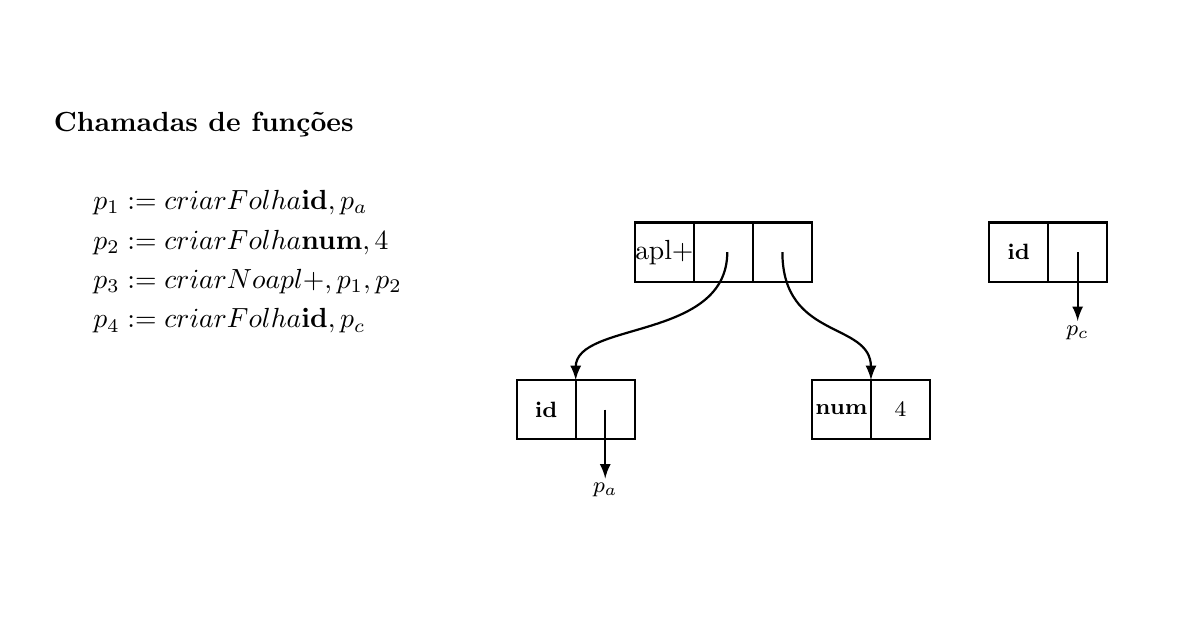
\begin{tikzpicture}
        \node[opacity=0] at (0, 0) { y };
        \node[opacity=0] at (14, 7) { t };

        \node[anchor=west] at (0, 6) { \textbf{Chamadas de funções} };
        \node[anchor=west] at (0.5, 5) { $p_1 := \Call{criarFolha}{\textbf{id}, p_a}$ };
        \node[anchor=west] at (0.5, 4.5) { $p_2 := \Call{criarFolha}{\textbf{num}, 4}$ };
        \node[anchor=west] at (0.5, 4) { $p_3 := \Call{criarNo}{\code{apl}{+}, p_1, p_2}$ };
        \node[anchor=west] at (0.5, 3.5) { $p_4 := \Call{criarFolha}{\textbf{id}, p_c}$ };

        \draw[thick] (6, 2) rectangle (6.75, 2.75);
        \node at (6.375, 2.375) { \footnotesize \textbf{id} };
        \draw[thick] (6.75, 2) rectangle (7.5, 2.75);
        \draw[thick,-latex] (7.125, 2.375) to (7.125, 1.5);
        \node at (7.125, 1.35) { \footnotesize $p_a$ };
        \draw[thick] (9.75, 2) rectangle (10.5, 2.75);
        \node at (10.125, 2.375) { \footnotesize \textbf{num} };
        \draw[thick] (10.5, 2) rectangle (11.25, 2.75);
        \node at (10.875, 2.375) { \footnotesize $4$ };
        \draw[thick] (7.5, 4) rectangle (8.25, 4.75);
        \node at (7.875, 4.375) { \code{apl}{+} };
        \draw[thick] (8.25, 4) rectangle (9, 4.75);
        \draw[-latex, thick] (8.675, 4.375) .. controls (8.675, 3.25) and (6.75, 3.5) .. (6.75, 2.75);
        \draw[thick] (9, 4) rectangle (9.75, 4.75);
        \draw[-latex, thick] (9.375, 4.375) .. controls (9.375, 3.25) and (10.5, 3.5) .. (10.5, 2.75);
%        \draw[thick] (9.75, 6) rectangle (10.5, 6.75);
%        \draw[thick] (10.5, 6) rectangle (11.25, 6.75);
%        \draw[thick] (11.25, 6) rectangle (12, 6.75);
        \draw[thick] (12, 4) rectangle (12.75, 4.75);
        \node at (12.375, 4.375) { \footnotesize \textbf{id} };
        \draw[thick] (12.75, 4) rectangle (13.5, 4.75);
        \draw[thick,-latex] (13.125, 4.375) to (13.125, 3.5);
        \node at (13.125, 3.35) { \footnotesize $p_c$ };

    \end{tikzpicture}

\end{frame}

\begin{frame}[fragile]{Criação da árvore sintática da expressão \code{apl}{a + 4 - c}}

    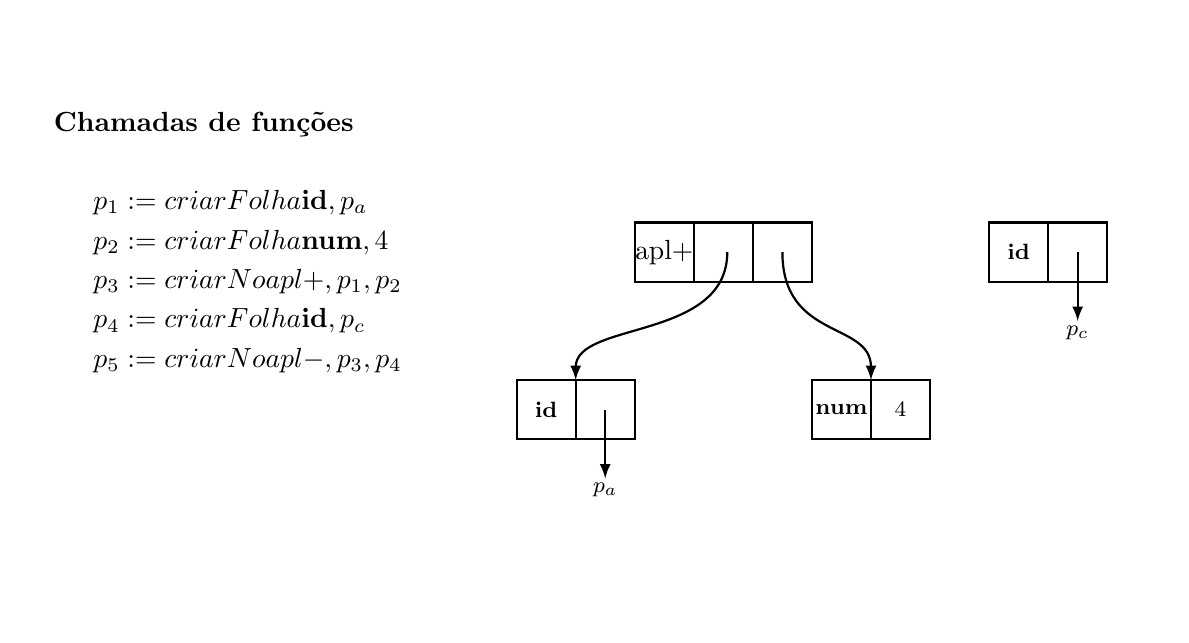
\begin{tikzpicture}
        \node[opacity=0] at (0, 0) { y };
        \node[opacity=0] at (14, 7) { t };

        \node[anchor=west] at (0, 6) { \textbf{Chamadas de funções} };
        \node[anchor=west] at (0.5, 5) { $p_1 := \Call{criarFolha}{\textbf{id}, p_a}$ };
        \node[anchor=west] at (0.5, 4.5) { $p_2 := \Call{criarFolha}{\textbf{num}, 4}$ };
        \node[anchor=west] at (0.5, 4) { $p_3 := \Call{criarNo}{\code{apl}{+}, p_1, p_2}$ };
        \node[anchor=west] at (0.5, 3.5) { $p_4 := \Call{criarFolha}{\textbf{id}, p_c}$ };
        \node[anchor=west] at (0.5, 3) { $p_5 := \Call{criarNo}{\code{apl}{-}, p_3, p_4}$ };

        \draw[thick] (6, 2) rectangle (6.75, 2.75);
        \node at (6.375, 2.375) { \footnotesize \textbf{id} };
        \draw[thick] (6.75, 2) rectangle (7.5, 2.75);
        \draw[thick,-latex] (7.125, 2.375) to (7.125, 1.5);
        \node at (7.125, 1.35) { \footnotesize $p_a$ };
        \draw[thick] (9.75, 2) rectangle (10.5, 2.75);
        \node at (10.125, 2.375) { \footnotesize \textbf{num} };
        \draw[thick] (10.5, 2) rectangle (11.25, 2.75);
        \node at (10.875, 2.375) { \footnotesize $4$ };
        \draw[thick] (7.5, 4) rectangle (8.25, 4.75);
        \node at (7.875, 4.375) { \code{apl}{+} };
        \draw[thick] (8.25, 4) rectangle (9, 4.75);
        \draw[-latex, thick] (8.675, 4.375) .. controls (8.675, 3.25) and (6.75, 3.5) .. (6.75, 2.75);
        \draw[thick] (9, 4) rectangle (9.75, 4.75);
        \draw[-latex, thick] (9.375, 4.375) .. controls (9.375, 3.25) and (10.5, 3.5) .. (10.5, 2.75);
%        \draw[thick] (9.75, 6) rectangle (10.5, 6.75);
%        \draw[thick] (10.5, 6) rectangle (11.25, 6.75);
%        \draw[thick] (11.25, 6) rectangle (12, 6.75);
        \draw[thick] (12, 4) rectangle (12.75, 4.75);
        \node at (12.375, 4.375) { \footnotesize \textbf{id} };
        \draw[thick] (12.75, 4) rectangle (13.5, 4.75);
        \draw[thick,-latex] (13.125, 4.375) to (13.125, 3.5);
        \node at (13.125, 3.35) { \footnotesize $p_c$ };

    \end{tikzpicture}

\end{frame}

\begin{frame}[fragile]{Criação da árvore sintática da expressão \code{apl}{a + 4 - c}}

    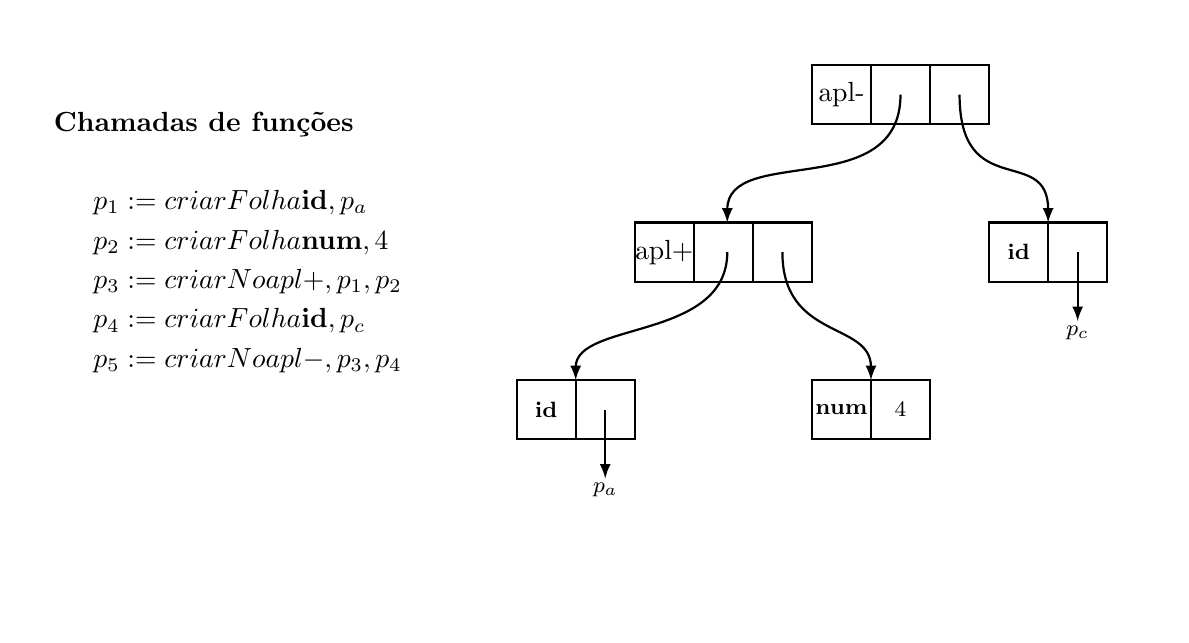
\begin{tikzpicture}
        \node[opacity=0] at (0, 0) { y };
        \node[opacity=0] at (14, 7) { t };

        \node[anchor=west] at (0, 6) { \textbf{Chamadas de funções} };
        \node[anchor=west] at (0.5, 5) { $p_1 := \Call{criarFolha}{\textbf{id}, p_a}$ };
        \node[anchor=west] at (0.5, 4.5) { $p_2 := \Call{criarFolha}{\textbf{num}, 4}$ };
        \node[anchor=west] at (0.5, 4) { $p_3 := \Call{criarNo}{\code{apl}{+}, p_1, p_2}$ };
        \node[anchor=west] at (0.5, 3.5) { $p_4 := \Call{criarFolha}{\textbf{id}, p_c}$ };
        \node[anchor=west] at (0.5, 3) { $p_5 := \Call{criarNo}{\code{apl}{-}, p_3, p_4}$ };

        \draw[thick] (6, 2) rectangle (6.75, 2.75);
        \node at (6.375, 2.375) { \footnotesize \textbf{id} };
        \draw[thick] (6.75, 2) rectangle (7.5, 2.75);
        \draw[thick,-latex] (7.125, 2.375) to (7.125, 1.5);
        \node at (7.125, 1.35) { \footnotesize $p_a$ };
        \draw[thick] (9.75, 2) rectangle (10.5, 2.75);
        \node at (10.125, 2.375) { \footnotesize \textbf{num} };
        \draw[thick] (10.5, 2) rectangle (11.25, 2.75);
        \node at (10.875, 2.375) { \footnotesize $4$ };
        \draw[thick] (7.5, 4) rectangle (8.25, 4.75);
        \node at (7.875, 4.375) { \code{apl}{+} };
        \draw[thick] (8.25, 4) rectangle (9, 4.75);
        \draw[-latex, thick] (8.675, 4.375) .. controls (8.675, 3.25) and (6.75, 3.5) .. (6.75, 2.75);
        \draw[thick] (9, 4) rectangle (9.75, 4.75);
        \draw[-latex, thick] (9.375, 4.375) .. controls (9.375, 3.25) and (10.5, 3.5) .. (10.5, 2.75);
        \draw[thick] (9.75, 6) rectangle (10.5, 6.75);
        \node at (10.125, 6.375) { \code{apl}{-} };
        \draw[thick] (10.5, 6) rectangle (11.25, 6.75);
        \draw[-latex, thick] (10.875, 6.375) .. controls (10.875, 5) and (8.675, 5.75) .. (8.675, 4.75);
        \draw[thick] (11.25, 6) rectangle (12, 6.75);
        \draw[-latex, thick] (11.625, 6.375) .. controls (11.625, 5) and (12.75, 5.75) .. (12.75, 4.75);
        \draw[thick] (12, 4) rectangle (12.75, 4.75);
        \node at (12.375, 4.375) { \footnotesize \textbf{id} };
        \draw[thick] (12.75, 4) rectangle (13.5, 4.75);
        \draw[thick,-latex] (13.125, 4.375) to (13.125, 3.5);
        \node at (13.125, 3.35) { \footnotesize $p_c$ };

    \end{tikzpicture}

\end{frame}
